\subsubsection{Mapping of meal and insulin features over time}

For creating time-dependent features from meal images and insulin intake doses, we employed a mechanistic modeling approach to represent human metabolism. This knowledge-based modeling framework allows us to incorporate established physiological principles and empirical findings into the feature creation process. We process six features: \textit{simple sugars}, \textit{complex sugars}, \textit{fats}, \textit{dietary fibers}, \textit{proteins}, and \textit{insulin}.

For this we begin by subtracting the intake time \( t_i \) from the current time \( t \) to obtain \( \Delta t = t - t_i \). The resulting \( \Delta t \) represents the elapsed time since the ingestion of the macronutrient or insulin. The relative impact of each compound on blood glucose change is then modeled using cubic Bezier curves defined by four control points.

A Bezier curve \( B(t) \) is a parametric curve that interpolates between control points using Bernstein polynomials as basis functions. For a set of \( n+1 \) control points \( P_0, P_1, \ldots, P_n \), the Bezier curve is defined as:

\begin{equation}
B(t) = \sum_{i=0}^{n} P_i \binom{n}{i} t^i (1-t)^{n-i}, \quad t \in [0,1]
\end{equation}

where \( \binom{n}{i} \) is the binomial coefficient and \( t \) is the parameter that traces the curve from \( t=0 \) to \( t=1 \). In our implementation, we use cubic Bezier curves (\( n=3 \)) with four control points \( P_0, P_1, P_2, P_3 \). The x-axis represents time in hours since ingestion/injection (\(\Delta t\)), and the y-axis represents the relative impact strength (normalized between 0 and 1).

For each macronutrient and insulin type, we define a unique set of control points, optimized per patient, to capture its metabolic characteristics. The control points are defined as follows:
\begin{itemize}
    \item \( P_0 = (0,0) \): Fixed at the origin, representing zero impact at intake time.
    \item \( P_1 = (x_1, y_1) \): Optimized coordinates influencing the initial rise.
    \item \( P_2 = (x_2, y_2) \): Optimized coordinates determining the peak impact and decay start.
    \item \( P_3 = (x_3, 0) \): Optimized x-coordinate \(x_3\) with a fixed y-coordinate of 0, marking the time point where the impact returns to zero.
\end{itemize}
The optimization process determines \(x_1, y_1, x_2, y_2, x_3\) for each feature, subject to constraints (e.g., \(0 < x_1 < x_2 < x_3\), specific ranges for x-coordinates, \(0.1 \le y_1 \le 1.0\), \(0.0 \le y_2 \le 1.0\)).

The weight of each intake at time \( t \) is determined by evaluating the corresponding optimized Bezier curve based on the elapsed time \( \Delta t \). First, the curve is generated by calculating numerous points along its path using the Bernstein polynomial definition. Then, for a given \( \Delta t \), if it falls within the time range covered by the curve's x-coordinates (from 0 to \( x_3 \)), we find the point on the generated curve whose x-coordinate is closest to \( \Delta t \). The y-coordinate of this point represents the relative impact weight at that elapsed time. If \( \Delta t \) is negative or exceeds the curve's duration (\(x_3\)), the weight is zero.

Once the feature values (impact weights multiplied by intake amounts) have been calculated and summed across all relevant prior intakes for a given time \(t\), we further adjust them by incorporating the prediction horizon. Specifically, the total weighted feature value calculated for the current time point is subtracted from the total weighted feature value calculated for the time point corresponding to the prediction horizon. This difference reflects the anticipated change in the cumulative feature impact over the forecast period, which is used as input for the predictive model. This adjustment ensures that the model accounts for the expected future impact dynamics of insulin and meal intakes on glucose levels.

\subsubsection{Bezier Curve Dynamics: Running Example}

\begin{figure}[h]
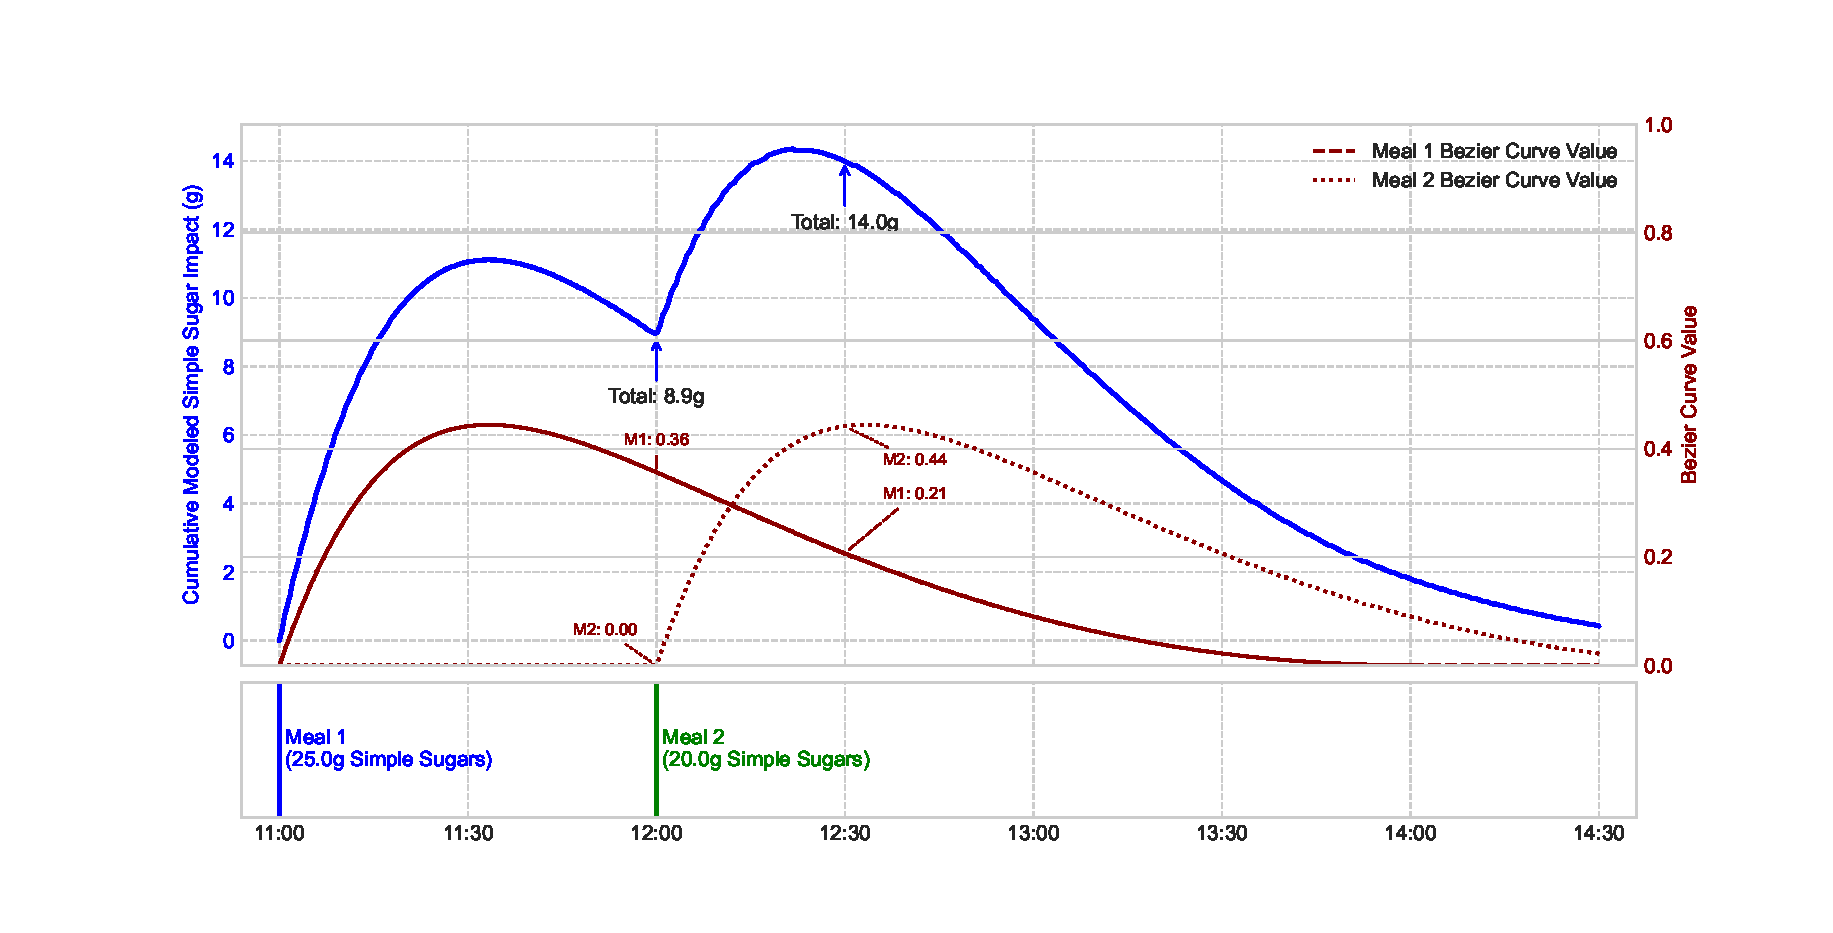
\includegraphics[width=\linewidth]{images/methods/example_bezier.eps}
\caption{Running example on how Bezier curve feature mapping is used to estimate the combined impact of macronutrients from different meals on blood glucose.}
\label{fig:bezier_curve}
\end{figure}

In our mechanistic model, we want to ensure that the ingested macronutrients are well modelled over time and that their combined impact from different meal intakes is considered. To illustrate how the Bezier curve modeling works in practice, we present a concrete example focusing on simple sugar intake from two meals.
Consider a patient who consumes two meals: Meal 1 at 11:00 AM containing 25g of \textit{simple sugars}, and Meal 2 at 12:00 PM containing 20g of \textit{simple sugars}. For \textit{simple sugars}, we use the patient-specific, optimized cubic Bezier curve. Let's assume for this patient, the optimized curve yields specific impact strengths at different elapsed times.

At 12:00 PM (\(t\)), we calculate the impact of both meals:
Meal 1 was 1 hour ago (\(\Delta t_1 = 1.0\)). Let's say the curve gives a relative impact strength of 0.55 at \(x=1.0\). The current impact is 25g × 0.55 = 13.75g of effective \textit{simple sugars}.
Meal 2 was just ingested (\(\Delta t_2 = 0.0\)). The relative impact strength is 0 (since \(P_0 = (0,0)\)). The current impact is 20g × 0 = 0g.
Thus, the total combined impact at 12:00 PM is 13.75g + 0g = 13.75g of effective \textit{simple sugars}.

30 minutes later at 12:30 PM (\(t\)):
Meal 1 was 1.5 hours ago (\(\Delta t_1 = 1.5\)). Let's assume the curve gives an impact strength of 0.35 at \(x=1.5\). The impact is 25g × 0.35 = 8.75g.
Meal 2 was 0.5 hours ago (\(\Delta t_2 = 0.5\)). Let's assume the curve gives an impact strength of 0.65 at \(x=0.5\). The impact is 20g × 0.65 = 13.0g.
The total combined impact at 12:30 PM is 8.75g + 13.0g = 21.75g of effective \textit{simple sugars}.

This demonstrates how the model aggregates impacts over time. If we were predicting with a horizon (e.g., 30 minutes), we would calculate this value at the current time and at the future time point, and use the difference as the feature value.

\subsubsection{Bezier Curve control point optimization}
To tailor our glucose prediction model to individual patient metabolism patterns, we implemented a patient-specific optimization approach for the Bezier curve control points. This personalization strategy improves prediction accuracy while providing valuable insights into each patient's unique metabolic response to different macronutrients and insulin types.

The optimization process leverages Optuna \cite{akiba2019optuna}, a hyperparameter optimization framework, with a Bayesian approach using Tree-structured Parzen Estimator (TPE) sampling. For each patient, we optimize the control points of the cubic Bezier curves for all six meal and insulin features (simple sugars, complex sugars, fats, dietary fibers, proteins, insulin).

Each cubic Bezier curve is defined by four control points \(P_0, P_1, P_2, P_3\). \(P_0\) is fixed at \((0,0)\) and \(P_3\) has a fixed y-coordinate of 0. This leaves five parameters to optimize for each curve: the coordinates of \(P_1\) (\(x_1, y_1\)), the coordinates of \(P_2\) (\(x_2, y_2\)), and the x-coordinate of \(P_3\) (\(x_3\)).

The optimization process employs several additional constraints to maintain physiologically plausible curve shapes:
(1) X-coordinates (time dimension) must be monotonically increasing (\( 0 < x_1 < x_2 < x_3 \)) to ensure temporal progression. (2) Y-coordinates \(y_1\) and \(y_2\) are constrained (\(0.1 \le y_1 \le 1.0\), \(0.0 \le y_2 \le 1.0\)). (3) For each of the six features, we selected literature-based boundaries for the x-coordinates \(x_1, x_2, x_3\) (representing onset, peak time, and duration). See Figure \ref{tab:feature_params} in the Supplementary Data for the exact parameter boundaries.

The optimization objective function aims to maximize the absolute Pearson correlation between the weighted sum of the generated feature impacts (using optimized weights for each feature type) and the actual observed glucose change over the first three days of data for each patient. For each trial, Optuna proposes new control point configurations (\(x_1, y_1, x_2, y_2, x_3\) for each feature) and feature weights within the defined constraints. The resulting Bezier curves generate feature values, which are then weighted and summed. The correlation between this sum and the target variable (normalized glucose change) is calculated, and the objective is to minimize \(1 - |\text{correlation}|\). We optimize across \( n_{trials}=300 \) iterations per patient using parallel processing with 6 workers to efficiently search the high-dimensional parameter space (30 parameters per patient across 6 features, plus 6 feature weights). 